\documentclass[9pt]{beamer}

\usepackage{amsfonts}
\usepackage{amsmath}
\usepackage{amssymb}
\usepackage{cuted}
\usepackage{hyperref}
\usepackage{mathtools}
\usepackage{multirow}
\usepackage{subcaption}

\usepackage{siunitx}
\DeclareSIUnit{\belmilliwatt}{Bm}
\DeclareSIUnit{\dBm}{\deci\belmilliwatt}

\usepackage{blindtext}
\newcommand\blfootnote[1]{%
\begingroup
\renewcommand\thefootnote{}\footnote{#1}%
\addtocounter{footnote}{-1}%
\endgroup
}

\usetheme{Warsaw}

\AtBeginSection
{
    \begin{frame}
        \frametitle{Table of Contents}
        \tableofcontents[currentsection]
    \end{frame}
}

\title[Waveform and Passive Beamforming Design for IRS-Aided SWIPT]{Waveform and Passive Beamforming Design for Intelligent Reflecting Surface-Aided Wireless Information and Power Transfer}
\author{Yang Zhao}
\institute{Department of Electrical and Electronic Engineering\\ Imperial College London}
\date{Early Stage Assessment, \today}

\begin{document}

\frame{\titlepage}

\begin{section}{Introduction and Review}
	\begin{subsection}{WPT}
		\begin{frame}{What is WPT?}
			\textbf{Wireless Power Transfer} (WPT) varies electromagnetic fields to deliver power.
			\vspace{1em}
			\begin{table}
				\scriptsize
				\caption{WPT Technologies}
				\begin{tabular}{|l|l|l|l|l|l|}
					\hline
					Categories                  & Technology                 & Devices           & Power                        & Frequency          & Range           \\ \hline
					\multirow{3}{*}{Near-field} & Magnetic resonant coupling & Resonators        & Up to 10 \si{\W}             & kHz -- MHz         & m               \\ \cline{2-6}
												& Inductive coupling         & Wire coils        & Up to 10 \si{\W}             & Hz -- MHz          & mm -- cm        \\ \cline{2-6}
												& Capacitive coupling        & Metal plates      & Up to 1 \si{\W}              & kHz -- MHz         & mm              \\ \hline
					\multirow{2}{*}{Far-field}  & \alert{RF waves}           & \alert{Rectennas} & \alert{\si{\uW} -- \si{\mW}} & \alert{MHz -- GHz} & \alert{m -- km} \\ \cline{2-6}
												& Light waves                & Lasers            & \si{\uW} -- \si{\mW}         & THz                & km              \\ \hline
				\end{tabular}
			\end{table}
			\vspace{1em}
			\textbf{Characteristics}:
			\begin{itemize}
				\item no wires and batteries
				\item everlasting, controllable, reliable, sustainable
			\end{itemize}
		\end{frame}

		\begin{frame}{WPT by RF waves}
			\textbf{Energy flow}: DC $\to$ RF $\to$ RF $\to$ DC
			\begin{figure}
				\centering
				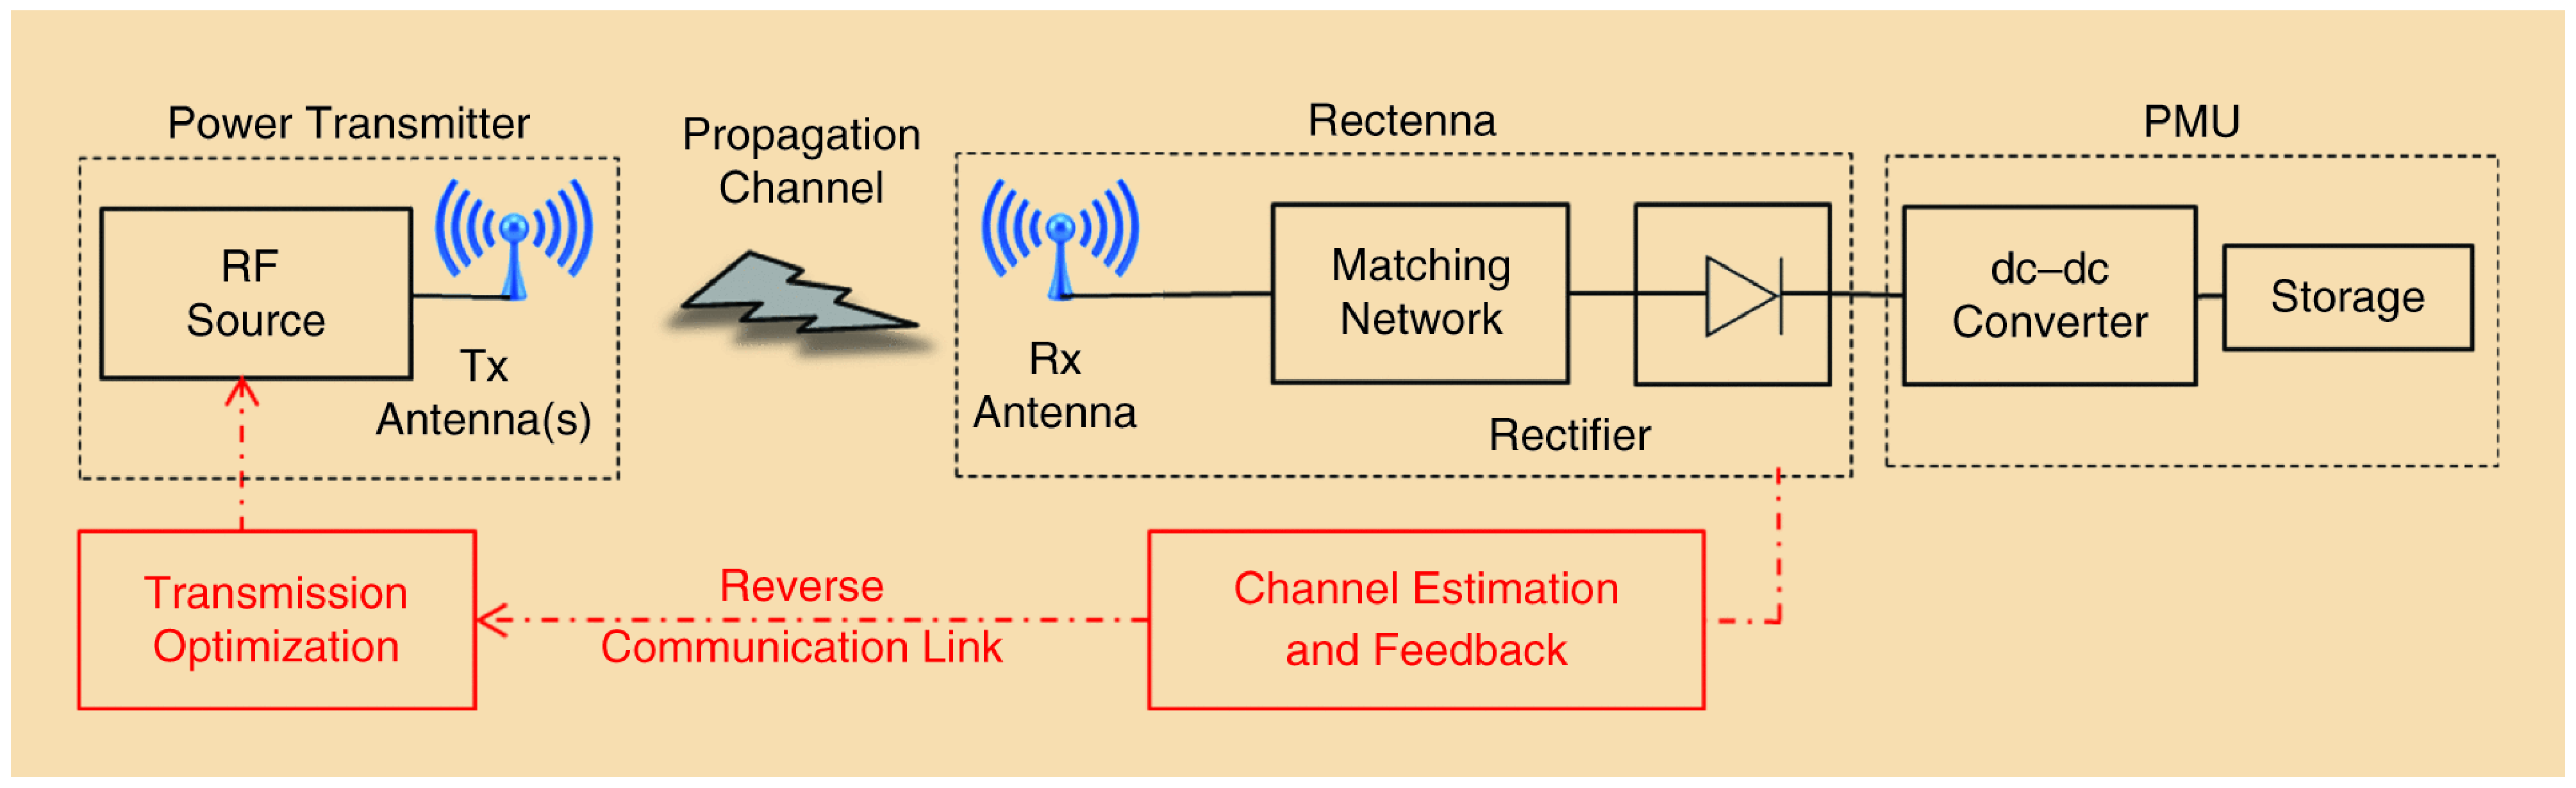
\includegraphics[width=\textwidth]{assets/wpt.eps}
			\end{figure}
			\textbf{Pros}:
			\begin{itemize}
				\item long range (up to hundreds of \si{\m}) with NLoS support
				\item compact receiver (few \si{\cm}), easy integration
				\item suitable for mobile devices
			\end{itemize}
			\textbf{Cons}:
			\begin{itemize}
				\item low power level (\si{\uW} -- \si{\mW})
				\item low energy harvesting efficiency (40\% at 100 \si{\uW}, 20\% at 10 \si{\uW})
			\end{itemize}
			\blfootnote{Figure from \cite{Clerckx2018a}}
		\end{frame}
	\end{subsection}

	\begin{subsection}{SWIPT}
		\begin{frame}{Why RF waves?}
			RF waves enables:
			\begin{itemize}
				\item Wireless communication (WIT)
				\item WPT
			\end{itemize}
			\vspace{1em}
			\textbf{Simultaneous Wireless Information and Power Transfer} (SWIPT): downlink WIT and WPT at the same time. Receivers can be either separated or \alert{co-located}.
			\vspace{1em}
			\begin{figure}
				\centering
				\begin{subfigure}{0.48\textwidth}
					\centering
					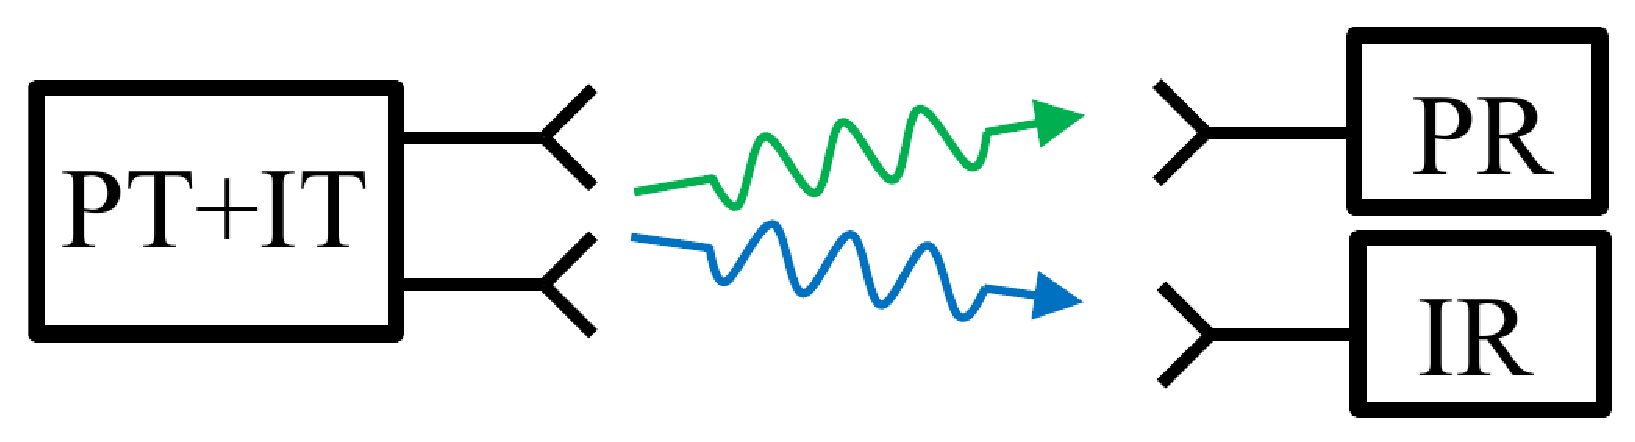
\includegraphics[width=0.8\linewidth]{assets/wipt_receiver_separated.eps}
					\caption{Separated}
				\end{subfigure}%
				\begin{subfigure}{0.48\textwidth}
					\centering
					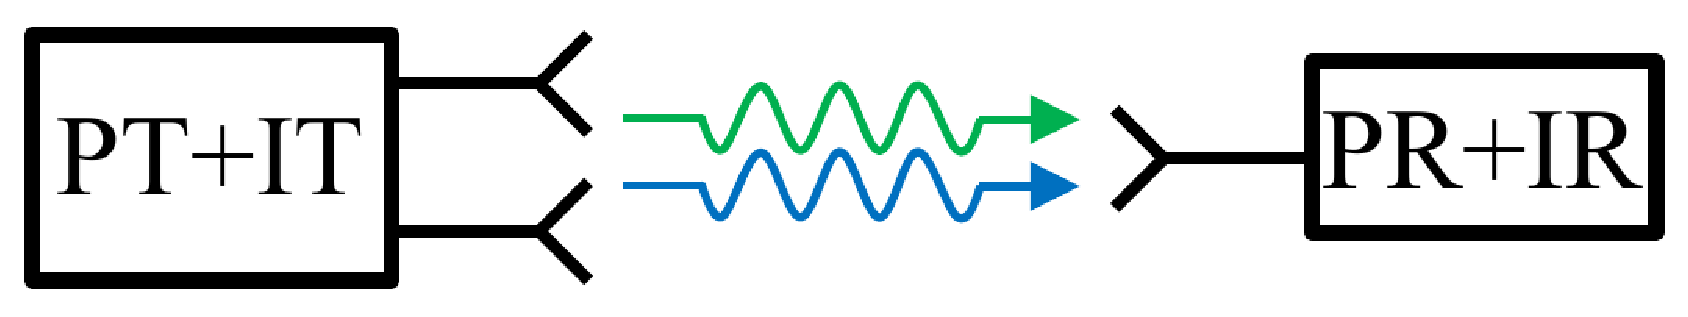
\includegraphics[width=0.8\linewidth]{assets/wipt_receiver_colocated.eps}
					\caption{Co-located}
				\end{subfigure}
				\caption{SWIPT receivers}
			\end{figure}
			\blfootnote{Figure from \cite{Clerckx2019}}
		\end{frame}

		\begin{frame}{Co-located receiver architecture}
			Two practical receiver architecture:
			\begin{itemize}
				\item \textbf{Time-Switching} (TS) switches between Information Decoding (ID) and Energy Harvesting (EH) modes on time basis.
				\item \textbf{Power-Splitting} (PS) splits the received signal into individual components for ID and EH.
			\end{itemize}
			\begin{figure}
				\centering
				\begin{subfigure}{0.48\textwidth}
					\centering
					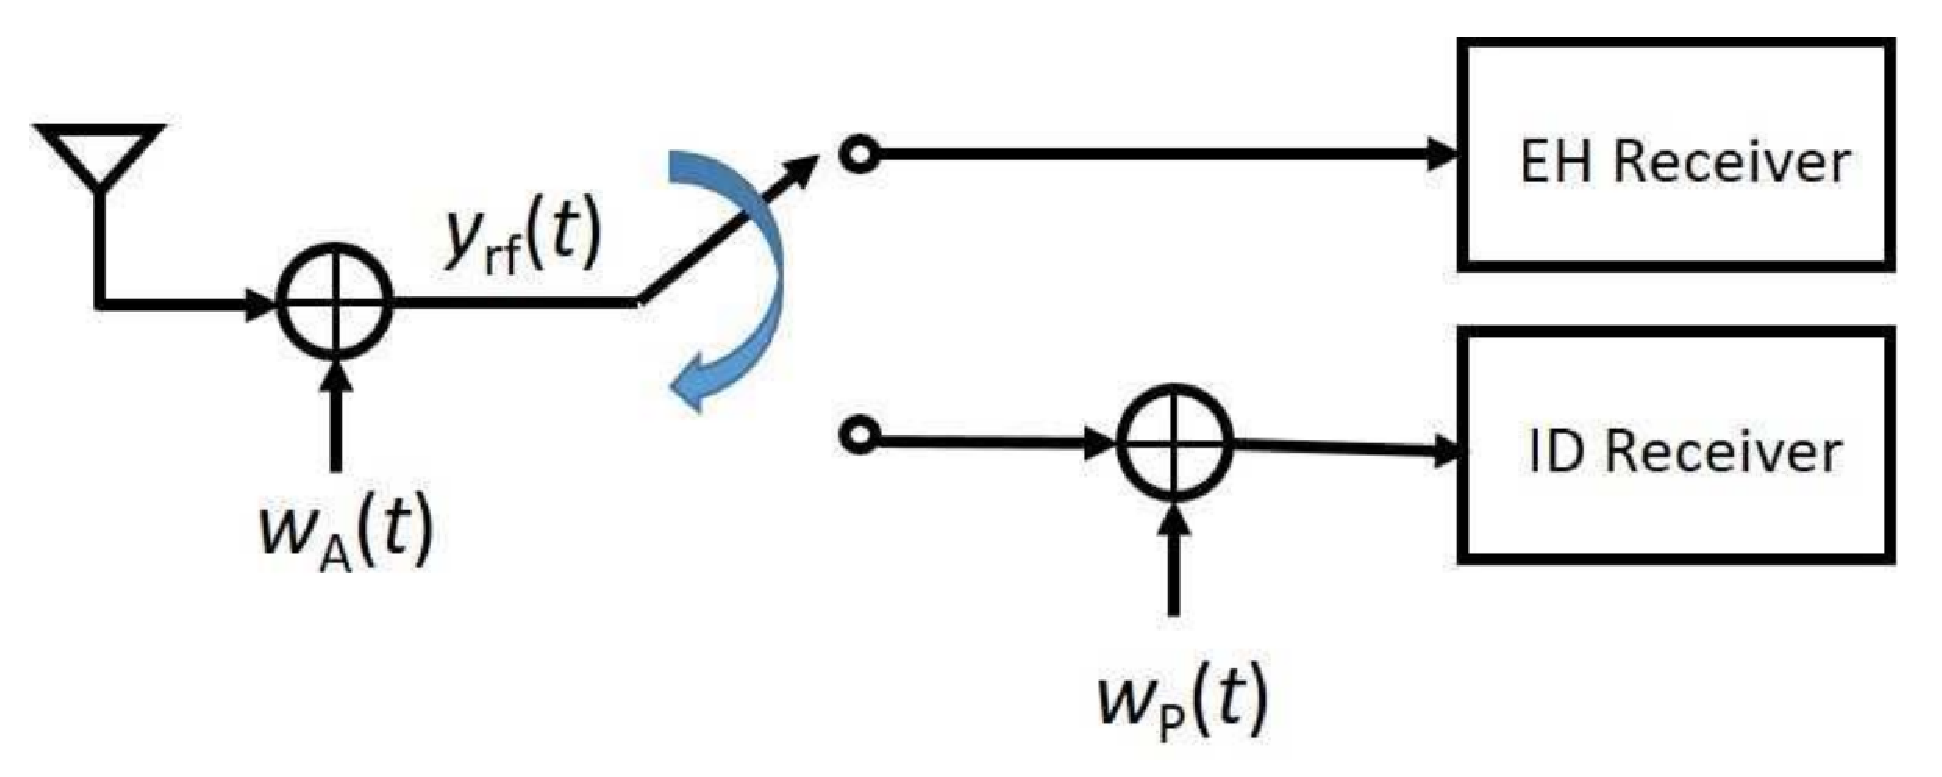
\includegraphics[width=0.8\linewidth]{assets/time_switching.eps}
					\caption{TS}
				\end{subfigure}%
				\begin{subfigure}{0.48\textwidth}
					\centering
					\includegraphics[width=0.8\linewidth]{assets/power_splitting.eps}
					\caption{PS}
				\end{subfigure}
				\caption{Co-located receiver architecture}
				\begin{block}{Design issue}
					\begin{itemize}
						\item TS can be achieved by a time sharing between WIT and WPT. Waveform is optimized individually for both cases.
						\item In PS, the splitting ratio $\rho$ is coupled with the waveform design.
					\end{itemize}
				\end{block}
			\end{figure}
			\blfootnote{Figure from \cite{Clerckx2019}}
		\end{frame}

		\begin{frame}{Harvester model}
			RF-to-DC conversion requires \textbf{rectenna} (receive antenna + rectifier), whose behavior is dominated by diode I-V characteristics.
			\begin{figure}
				\centering
				\includegraphics[width=0.8\textwidth]{assets/rectenna_circuit.eps}
				\caption{Rectenna equivalent circuit and a single diode rectifier \cite{Clerckx2018a}}
			\end{figure}
			Consider small-signal model and truncate its Taylor expansion to the $n_0$-th order:
			\begin{itemize}
				\item diode linear model (${n_o} = 2$): output power is proportional to input power
				\item \alert{diode nonlinear model} (${n_o} > 2$): significant contribution from high-order terms
			\end{itemize}
		\end{frame}

		\begin{frame}{Waveform design}
			A superposed signal containing \alert{modulated information waveform} and \alert{multisine power waveform} is demonstrated to bring a two-fold benefit:
			\begin{itemize}
				\item \textbf{rate}: multisine is deterministic with no interference on information waveform (by waveform cancellation or translated codebook)
				\item \textbf{energy}: multisine brings high PAPR and triggers the diode nonlinear model more often (reduce threshold from -20 \si{\dBm} to -30 \si{\dBm})
			\end{itemize}
			\begin{figure}
				\centering
				\begin{subfigure}{.48\textwidth}
					\centering
					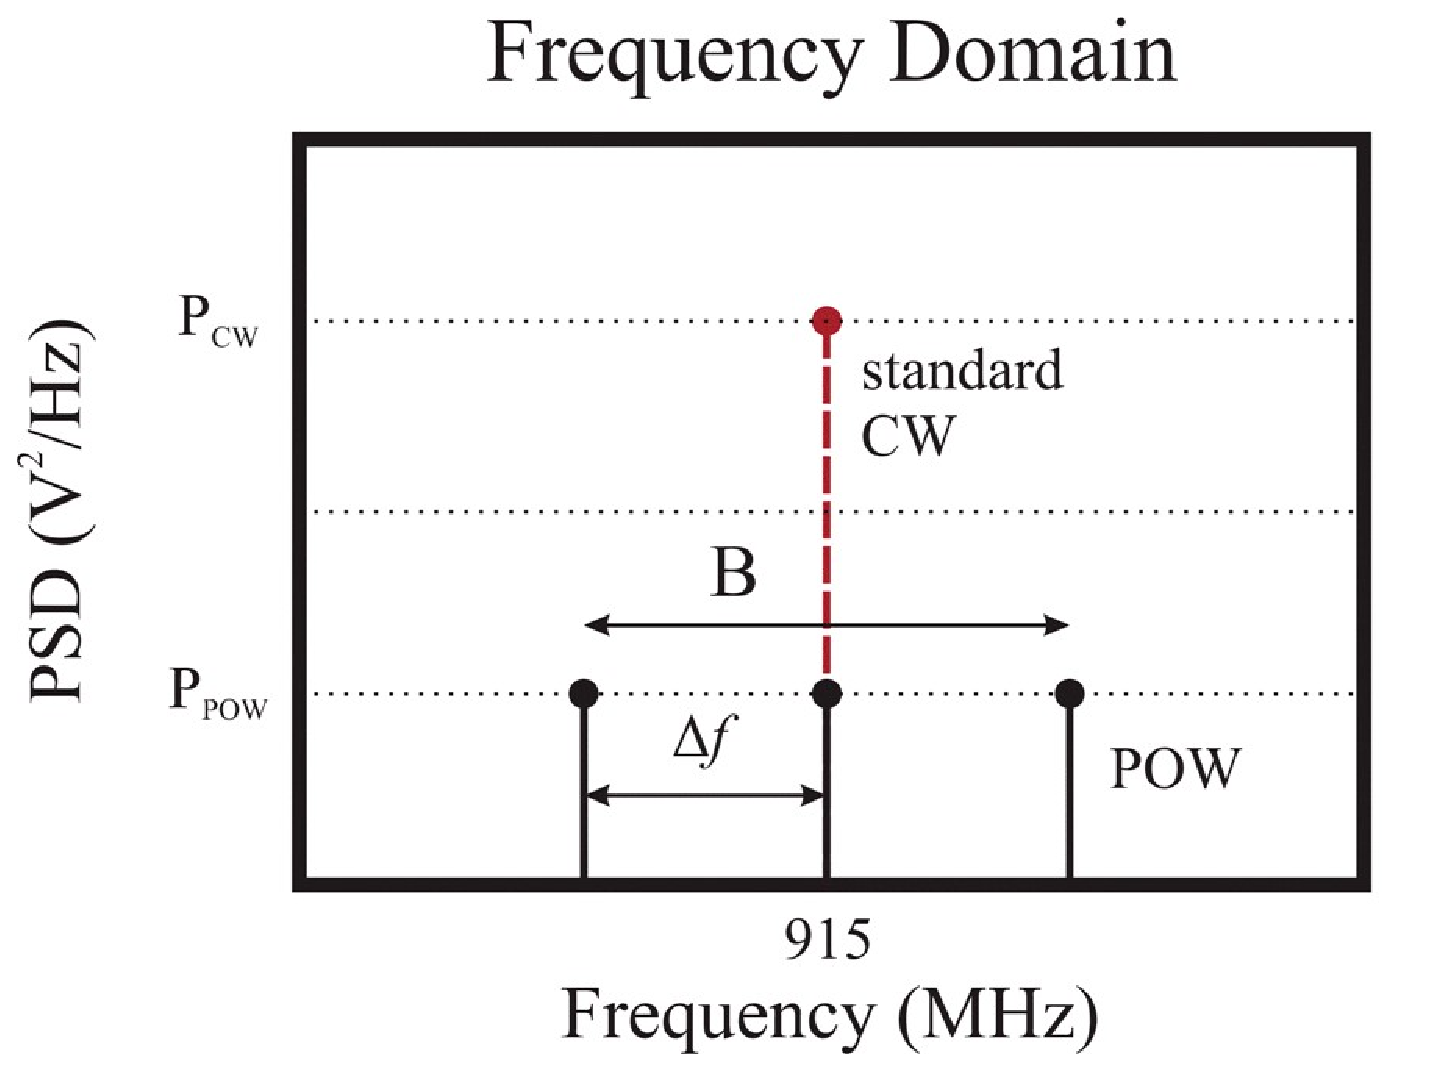
\includegraphics[width=0.8\linewidth]{assets/multisine_frequency_domain.eps}
					\caption{Frequency domain}
				\end{subfigure}
				\begin{subfigure}{.48\textwidth}
					\centering
					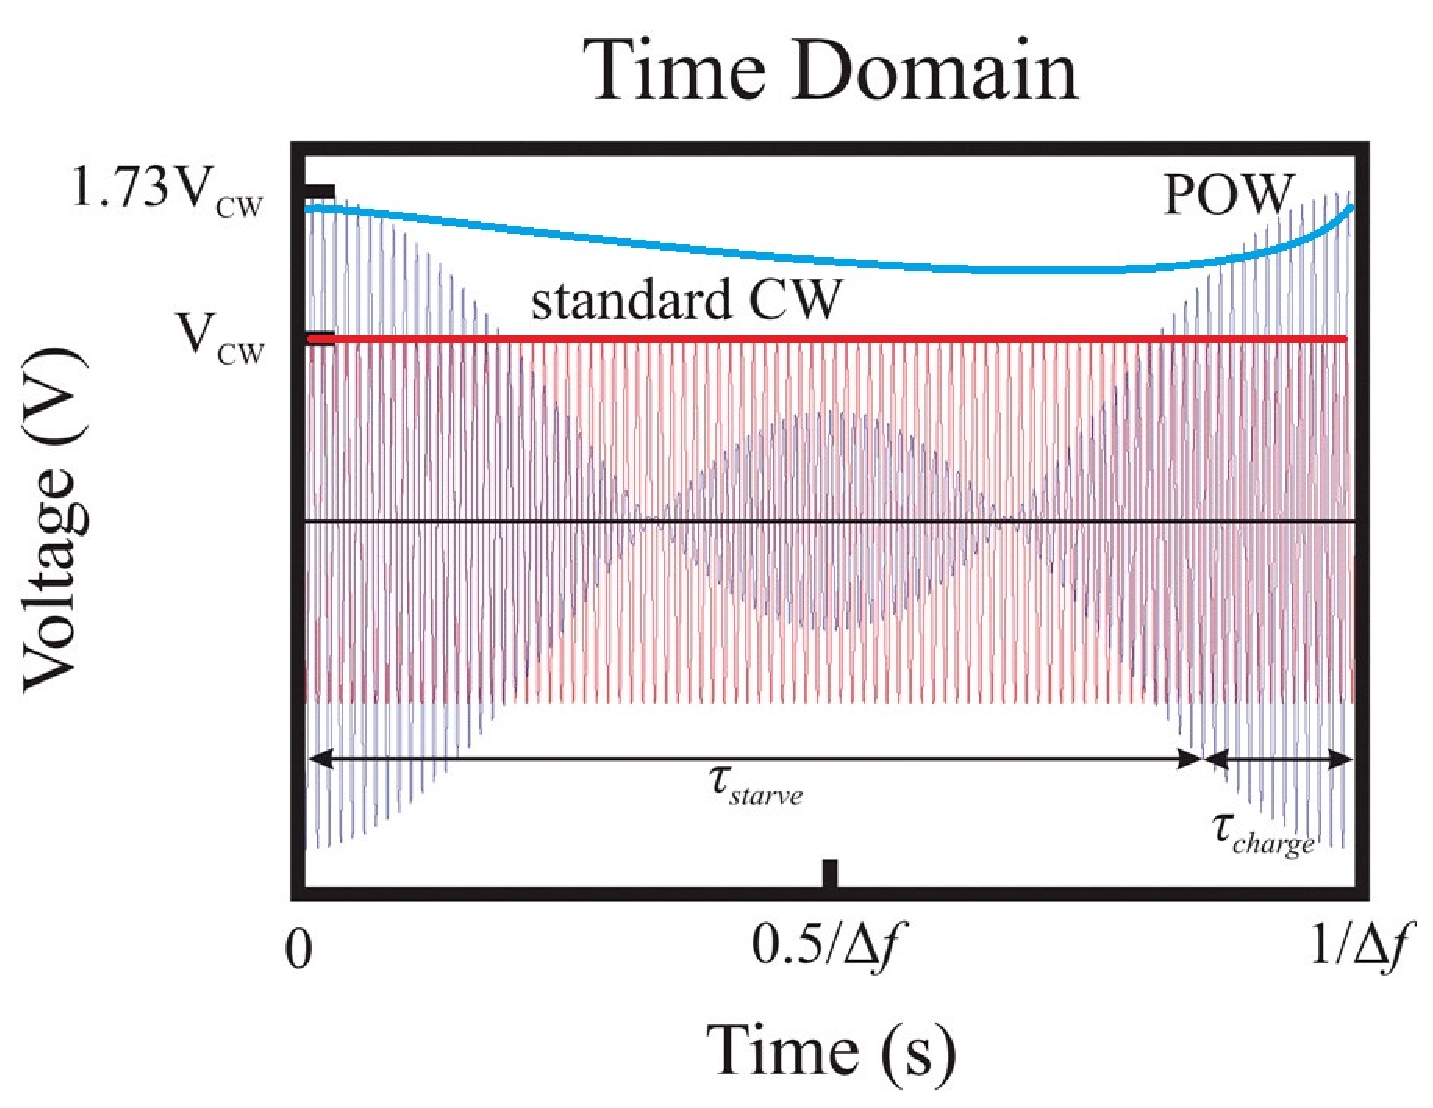
\includegraphics[width=0.8\linewidth]{assets/multisine_time_domain.eps}
					\caption{Time domain}
				\end{subfigure}
				\caption{Multisine waveform}
			\end{figure}
			\blfootnote{Figure from \cite{Trotter2009}}
		\end{frame}
	\end{subsection}

	\begin{subsection}{IRS}
		\begin{frame}{What is IRS?}
			\textbf{Intelligent Reflecting Surface} (IRS) consists of multiple individual passive reflecting elements that adjust the amplitude and phase of the incident signal.
			\begin{figure}
				\centering
				\begin{subfigure}{.48\textwidth}
					\centering
					\includegraphics[width=0.9\linewidth]{assets/irs_architecture.eps}
					\caption{IRS architecture}
				\end{subfigure}
				\begin{subfigure}{.48\textwidth}
					\centering
					\includegraphics[width=0.9\linewidth]{assets/irs_system.eps}
					\caption{Application scenario}
				\end{subfigure}
			\end{figure}
			\begin{columns}
				\begin{column}{0.5\textwidth}
					\begin{itemize}
						\item outer layer: redistribute incident signals
						\item middle layer: avoid signal energy leakage
						\item inner layer: adjust reflection amplitude and phase shift
					\end{itemize}
				\end{column}
				\begin{column}{0.5\textwidth}
					\begin{itemize}
						\item enhance primary transmission by constructive reflection
						\item null interference by destructive reflection
					\end{itemize}
				\end{column}
			\end{columns}
			\blfootnote{Figure from \cite{Wu2019,Wu2020}}
		\end{frame}

		\begin{frame}{Why IRS?}
			\textbf{Characteristics}:
			\begin{itemize}
				\item passive (different from AF relay)
				\begin{itemize}
					\item no RF chains
					\item low power consumption
					\item no additional thermal noise
					\item \alert{squared gain}: received power scales quadratically with the number of reflectors (boost receive power and array gain in equal gain transmission)
				\end{itemize}
				\item full-duplex
				\item assistant (different from backscatter node)
				\item adjustable in real-time
			\end{itemize}
			\vspace{1em}
			\textbf{Challenges}:
			\begin{itemize}
				\item channel estimation
				\begin{itemize}
					\item cannot separate incident and reflective channels
					\item large number of extra channels
				\end{itemize}
				\item practical restriction
				\begin{itemize}
					\item discrete phase shifts
					\item phase shift are coupled with reflection amplitude (by impedance equation)
				\end{itemize}
			\end{itemize}
		\end{frame}

		\begin{frame}{Why IRS-aided SWIPT?}
			\begin{itemize}
				\item both aim at improving spectral/energy efficiency
				\item enhanced channel boosts received power to benefit from harvester nonlinearity
				\item extra links increase system diversity and stability, which is essential for SWIPT
				\item SWIPT can potentially support low-power IRS
			\end{itemize}
		\end{frame}
	\end{subsection}
\end{section}

\bibliographystyle{IEEEtran}
\bibliography{library.bib}
\end{document}
